\section{Experiments}
In this section, we evaluate the model’s inference efficiency as well as its multi-frame integration ability. We further present ablation studies of the key components of our method and analyze the model’s behavior through attention-map visualizations.


\subsection{Acceleration}
In this study, we validate our method's performance under acceleration by enabling KV caching of static components. 

\noindent\textbf{Baselines}
For baselines, we compare to those that also adopt temporal information reuse. \emph{FlashVLA} \cite{tan2025think} simply reuses the previous action based on a heuristic criterion.
\emph{TTF-VLA} \cite{liu2025ttf} and \emph{VLA-cache} \cite{xu2025vla} identify reusable visual patches using hand-designed heuristics and cache the corresponding embeddings from previous steps; however, these cached patches are not guaranteed to remain static in the hidden representation space. All methods are based on the same VLA base model (i.e., CogACT~\cite{li2024cogact}), with all other necessary variables controlled consistently.

% \begin{table*}[]
% \newcolumntype{M}{>{\raggedleft\arraybackslash}p{0.1\linewidth}}
% \newcommand{\cchead}[1]{\multicolumn{1}{c}{#1}}
%     \centering\textbf{}
% \caption{Results on the SimplerEnv benchmark.}
% \label{tab:simplerenv}
%     \resizebox{\linewidth}{!}{
% \begin{tabular}{l|l|ccccc|ccc}
% \toprule
%  Google Robot & Method & PickCan & MoveNear & Drawer & DrawerApple & Average & FLOPs & Latency (ms) & Speedup \\
%  \midrule
%  \multirow{5}{*}{\makecell{SIMPLER\\ (Visual Matching)}}
%  & CogACT \cite{li2024cogact} & $91.3$ & $85.0$ & $71.8$ & $50.9$ & $74.8$ & 100\% & $339$ & $1.00\times$ \\
%   & + FlashVLA \cite{tan2025think} & $80.0$ & $57.1$ & $73.6$ \\
%  % RT-1 & 85.7 & 44.2 & 73.0 & 6.5 & 52.4 & NA \\
%  % & RT-1-X & 56.7 & 31.7 & 59.7 & 21.3 & 42.4 \\
%  % & RT-2-X  & 78.7 & 77.9 & 25.0 & 3.7 & 46.3 & NA \\
%  % & Octo-Base  & 17.0 & 4.2 & 22.7 & 0.0 & 11.0 & NA \\
%  % & OpenVLA  & 18.0 & 56.3 & 63.0 & 0.0 & 34.3 & NA \\
%  & + TTF \cite{liu2025ttf} & $89.3$ & $71.3$ & $58.4$  \\
%  & + VLA-Cache \cite{xu2025vla} &  $92.0$ & $85.0$  & $70.5$ & $51.6$ & & $80.1\%$ \\
%  % & EfficientVLA & 93.3 & 81.3 & 68.2 & 53.8 & 28.9\% \\
%  & + \dysta{} (Ours) & $92.7$ & $88.8$ & $75.0$ & $47.2$ & & $40.2\%$ & $151$ \\
%  \midrule
%  \multirow{5}{*}{\makecell{SIMPLER\\ (Variant Aggregation)}}
%  & CogACT \cite{li2024cogact} & $89.6$ & $80.8$ & $28.3$ & $46.6$ & $61.3$ \\
%  & + FlashVLA \cite{tan2025think} & $82.5$ & $60.8$ & $28.6v$\\
%  % & RT-1 [7] & 89.8 & 50.0 & 32.3 & 2.6 & 43.7 \\
%  % & RT-1-X [48] & 49.0 & 32.3 & 29.4 & 10.1 & 30.2 \\
%  % & RT-2-X [48] & 82.3 & 79.2 & 35.3 & 20.6 & 54.4 \\
%  % & Octo-Base [62] & 0.6 & 3.1 & 1.1 & 0.0 & 1.2 \\
%  % & OpenVLA [30] & 60.8 & 67.7 & 28.8 & 0.0 & 39.3 \\
%  & + TTF \cite{liu2025ttf} & $88.0$ & $62.7$ & $34.0$ \\
%  & + VLA-Cache \cite{xu2025vla} & $91.7$ & $79.3$  & $32.5$ & $45.8$ & \\
%  % & EfficientVLA & 93.2 & 75.8 & 26.9 & 49.2 & \\
%  & + \dysta{} (Ours) & $92.4$ & $81.0$ & $38.9$ & $46.0$ & \\
%  \bottomrule
% \end{tabular}
% }
% \end{table*}


% \begin{table*}[t]
% \newcolumntype{M}{>{\raggedleft\arraybackslash}p{0.1\linewidth}}
% \newcommand{\cchead}[1]{\multicolumn{1}{c}{#1}}
%     \centering\textbf{}
% \caption{Results on the SimplerEnv benchmark. Task suites follows the setting of \citet{qu2025spatialvla}.}
% \label{tab:simplerenv}
%     \resizebox{\linewidth}{!}{
% \begin{tabular}{l|cccccccc|ccc}
% \toprule
% \multirow{3}{*}{Method} & \multicolumn{4}{c}{Visual Matching} & \multicolumn{4}{c}{Variant Aggregation} & \multicolumn{3}{c}{Acceleration}  \\
% \cmidrule(lr){2-5}\cmidrule(lr){6-9}\cmidrule(lr){10-12}
% & \makecell{Pick\\Can} & \makecell{Move\\Near} & Drawer & \makecell{Drawer\\Apple} & \makecell{Pick\\Can}  & \makecell{Move\\Near} & Drawer & \makecell{Drawer\\Apple}   & FLOPs & \makecell{Latency\\(ms)} & Speedup \\
%  \midrule
%  CogACT \cite{li2024cogact} & $91.3$ & $85.0$ & $71.8$ & $50.9$ &$89.6$ & $80.8$ & $28.3$ & $46.6$  & 100\% & $1355$ & $1.00\times$ \\
%   + FlashVLA \cite{tan2025think} & $80.0$ & $57.1$ & $73.6$ & & $82.5$ & $60.8$ & $28.6$ &\\
%  + TTF \cite{liu2025ttf} & $89.3$ & $71.3$ & $58.4$ & & $88.0$ & $62.7$ & $34.0$ & \\
%  + VLA-Cache \cite{xu2025vla} &  $92.0$ & $83.3$  & $70.5$ &  & $91.7$ & $79.3$  & $32.5$ & $45.8$ & $80.1\%$ \\
%  + \dysta{} (Ours) & $\mathbf{92.7}$ & $\mathbf{88.8}$ & $\mathbf{75.0}$ & $47.2$ & $\mathbf{92.4}$  & $\mathbf{81.0}$ & $\mathbf{38.9}$ & $46.0$& $43.4\%$ & $577$ & $2.35\times$ \\
%  \bottomrule
% \end{tabular}
% }
% \end{table*}


\begin{table}[t]
\newcolumntype{M}{>{\raggedleft\arraybackslash}p{0.1\linewidth}}
\newcommand{\cchead}[1]{\multicolumn{1}{c}{#1}}
    \centering\textbf{}
\caption{Results on the SimplerEnv benchmark. Task suites follow the setting of \citet{qu2025spatialvla}. All baselines and our method are applied to the same VLA base model (i.e., CogACT~\cite{li2024cogact}).}
\label{tab:simplerenv}
    \resizebox{\linewidth}{!}{
\begin{tabular}{lcccccc|ccc}
\toprule
\multirow{3}{*}{Method} & \multicolumn{3}{c}{Visual Matching} & \multicolumn{3}{c}{Variant Aggregation} & \multicolumn{3}{c}{Acceleration}  \\
\cmidrule(lr){2-4}\cmidrule(lr){5-7}\cmidrule(lr){8-10}
& \makecell{Pick\\Can} & \makecell{Move\\Near} & Drawer & \makecell{Pick\\Can}  & \makecell{Move\\Near} & Drawer  & FLOPs & \makecell{Latency\\(ms)} & Speedup \\
 \midrule
  % RT-2-X \cite{vuong2023open} & $78.7$ & $77.9$ & $25.0$ & $82.3$ & $79.2$ & $35.3$ & $-$ & $-$ & $-$\\
  % Octo-Base \cite{team2024octo} & $17.0$ & $4.2$ & $22.7$ & $0.6$ & $3.1$ & $1.1$ & $-$ & $-$ & $-$ \\
  % OpenVLA \cite{kim2024openvla}  & $18.0$ & $56.3$ & $63.0$ & $60.8$ & $67.7$ & $28.8$ & $-$ & $-$ & $-$ \\
  % SpatialVLA \cite{qu2025spatialvla} & $81.0$ & $69.6$ & $59.3$ & $89.5$ & $71.7$ & $36.2$ & $-$ & $-$ & $-$ \\
  % $\pi_0$ \cite{black2024pi0visionlanguageactionflowmodel} & $88.0$ & $80.3$ & $56.0$ & $-$ & $-$ & $-$ & $-$ & $-$ & $-$ \\
  % \midrule
 CogACT \cite{li2024cogact} & $91.3$ & $\underline{85.0}$ & $71.8$ &$89.6$ & $\underline{80.8}$ & $28.3$  & 100\% & $1360$ & $1.00\times$ \\
  + FlashVLA \cite{tan2025think} & $80.0$ & $57.1$ & $\underline{73.6}$ & $82.5$ & $60.8$ & $28.6$ & $83.4\%$ & $1024$ & $1.33\times$\\
 + TTF \cite{liu2025ttf} & $89.3$ & $71.3$ & $58.4$ & $88.0$ & $62.7$ & $\underline{34.0}$ & $86.5\%$ & $1051$ & $1.29\times$  \\
 + VLA-Cache \cite{xu2025vla} &  $\underline{92.0}$ & $83.3$  & $70.5$ & $\underline{91.7}$ & $79.3$  & $32.5$ & $80.1\%$ & $985$ & $1.38\times$ \\
 + \dysta{} (Ours) & $\mathbf{92.7}$ & $\mathbf{88.8}$ & $\mathbf{75.0}$ & $\mathbf{92.4}$  & $\mathbf{81.0}$ & $\mathbf{38.9}$ & $\mathbf{43.4\%}$ & $\mathbf{601}$ & $\mathbf{2.26\times}$ \\
 \bottomrule
\end{tabular}
}
\end{table}


\begin{table}[t]
\centering
\caption{Results on the LIBERO benchmark. Policy inputs: third-person image, language instruction. All baselines and our method are applied to the same VLA base model (i.e., OpenVLA-OFT~\cite{kim2025fine}).}
\label{tab:libero}
\resizebox{\linewidth}{!}{
\begin{tabular}{lccccc|ccc}
\toprule
Models & Spatial & Object & Goal & Long & Average & FLOPs & Latency (ms) & Speedup \\
\midrule
% Diffusion Policy \cite{chi2025diffusion} & 78.3 & 92.5 & 68.3 & 50.5 & 72.4 & $-$ & $-$& $-$ \\
% Octo \cite{team2024octo} & 78.9 & 85.7 & 84.6 & 51.1 & 75.1 & $-$ & $-$& $-$\\
% DiT Policy \cite{hou2410diffusion} & 84.2 & 96.3 & 85.4 & 63.8 & 82.4 & $-$ & $-$& $-$\\
% OpenVLA \cite{kim2024openvla} & 84.7 & 88.4 & 79.2 & 53.7 & 76.5 & $-$ & $-$& $-$\\
% \midrule
OpenVLA-OFT \cite{kim2025fine} & $\underline{96.2}$ & $\mathbf{98.3}$ & $\mathbf{96.2}$ & $\underline{90.7}$ & $\underline{95.4}$ & $100.0\%$ & $741$ & $1.00\times$\\
% \midrule
+ FlashVLA \cite{tan2025think} & $71.8$ & $90.0$ &  $79.2$& $78.8$ & $80.0$ &  $88.7\%$& $657$ & $1.13\times$  \\
+ TTF \cite{liu2025ttf} & $95.8$ & $94.2$ &   $93.6$ &  $86.0$  & $92.4$ & $75.0\%$ & $575$ & $1.29\times$\\
% EfficientVLA & & & & 89.8 & \\
+ VLA-Cache \cite{xu2025vla} & $95.6$ & $92.8$ & $94.0$ & $89.6$ & $93.0$ & $85.5\%$ & $652$ & $1.14\times$ \\
+ \dysta{} (Ours) & $\mathbf{97.8}$ & $\underline{97.6}$ & $\mathbf{96.2}$ & $\mathbf{92.4}$ & $\mathbf{96.0}$ & $\mathbf{63.4}\%$ & $\mathbf{437}$ & $\mathbf{1.70}\times$ \\
\bottomrule
\end{tabular}
}
\end{table}

\noindent\textbf{Simulation benchmark}
We use SimplerEnv~\cite{li2024evaluating} and LIBERO~\cite{liu2023libero} task suite to evaluate the performance and acceleration. \citet{kim2025fine} offers two settings for LIBERO, one using only a third-person image and a language instruction as inputs, and another that additionally includes an extra camera view and proprioceptive state. We adopt the former setting, as it offers broader applicability and aligns more closely with standard VLA deployment scenarios. For the LIBERO benchmark, we finetune the model to the corresponding downstream datasets. For the SimplerEnv benchmark, we use Open X-Embodiment (OXE) \cite{vuong2023open} as the training dataset. All settings are consistent with the corresponding original base model.

\noindent\textbf{Real-World benchmark} We evaluate \dysta{} with Cobot Magic robots on 7 tasks across 3 categories, each with 20 trials. This evaluation scale is consistent with prior work~\cite{shi2025memoryvlaperceptualcognitivememoryvisionlanguageaction,li2024cogact}.

\noindent\textbf{Evaluation} The performance is measured by success rate, and acceleration is measured by the FLOPs reduction rate and the inference latency.

\noindent\textbf{Implementation details} We use two levels of static cache. L1 static cache consists of 133 ($52\%$) tokens and L2 static cache consists of 107 ($42\%$) tokens, resulting in 16 dynamic tokens. FLOPs are measured by open-source tools \footnote{\url{https://github.com/MrYxJ/calculate-flops.pytorch}}.

\noindent\textbf{Results}
Table~\ref{tab:simplerenv}  and Table~\ref{tab:libero} summarize the performance and the acceleration results. Table~\ref{tab:real_res} summarizes the results on the real-world benchmark. Across tables, we show that our method achieves improved or comparable performance across benchmarks with substantial speedup. Notably, on the SimplerEnv benchmark, our method improves the base model by $4.9\%$, and outperforms the best baseline by $3.9\%$ and achieves $2.26\times$ acceleration.  On the real-world benchmark, our model improves the base model by $10.6\%$ and achieves $2.21\times$ acceleration.

\subsection{Multi-Frame Integration for Temporal-dependency Modeling} 

\noindent\textbf{Baselines}
We consider the following baselines: \emph{OpenVLA-OFT$^\dagger$} incorporates full image tokens from historical observations. Since this baseline incurs a prohibitively large context length compared with standard models, we allocate the maximum available resources and tune it for the best achievable performance. \emph{TTF-VLA} \cite{liu2025ttf} mixes the current observation with past observations in a patch-wise manner. \emph{TraceVLA} \cite{zheng2024tracevla} visualizes the trajectories of active points by overlaying them onto the image using distinct colors, referred to as visual traces. \emph{MemoryVLA} \cite{shi2025memoryvlaperceptualcognitivememoryvisionlanguageaction} feeds the LLM backbone with images from each timestep independently and extracts a representation for each; only the multi-timestep representations are provided to the decoder. \emph{ContextVLA} \cite{jang2025contextvla} pools historical observations into a fixed number of tokens and prepends them to the image tokens of the current observation. All methods are applied to the same VLA base model (i.e., OpenVLA-OFT~\cite{kim2025fine}), with all other necessary variables controlled consistently.


\begin{table}[t]
\centering
\caption{Success rate (\%) on real-world experiments with the Cobot Magic robot. All baselines and our method are applied to the same VLA base model (i.e., OpenVLA-OFT~\cite{kim2025fine}).}
\label{tab:real_res}
\resizebox{\linewidth}{!}{
\begin{tabular}{l|cccc|cc|c|ccc}
\toprule
\multirow{3}{*}{Method}
& \multicolumn{4}{c|}{Pick-and-Place}
& \multicolumn{2}{c|}{Pouring}
& \multicolumn{1}{c|}{Container}
& \multicolumn{3}{c}{Acceleration Metrics} \\
\cmidrule(lr){2-5}
\cmidrule(lr){6-7}
\cmidrule(lr){8-8}
\cmidrule(lr){9-11}

& \makecell{Corn\\$\rightarrow$Pot}
& \makecell{Corn\\$\rightarrow$Plate}
& \makecell{Bread\\$\rightarrow$Pan}
& \makecell{Carrot\\Transfer}
& \makecell{Pour\\Coke}
& \makecell{Pour\\Bottle}
& \makecell{Open\\Drawer}
& FLOPs
& \makecell{Latency\\(ms)}
& Speedup \\
\midrule

OpenVLA-OFT
& $55$ & $\underline{70}$ & $\mathbf{55}$ & $\underline{65}$
& $\underline{60}$ & $35$
& $\mathbf{35}$
& $100.0\%$
& $1089$
& $1.00\times$ \\

+ FlashVLA
& $35$ & $55$ & $30$ & $50$
& $55$ & $30$
& $15$
& $\underline{62.5\%}$
& $\underline{791}$
& $\underline{1.30\times}$ \\

+ TTF
& $35$ & $\underline{70}$ & $30$ & $55$
& $55$ & $\underline{40}$
& $15$
& $98.6\%$
& $1077$
& $1.01\times$ \\

+ VLA-Cache
& $\underline{60}$ & $65$ & $35$ & $50$
& $45$ & $\underline{40}$
& $30$
& $74.0\%$
& $836$
& $1.27\times$ \\

% \midrule
+ \dysta{} (Ours)
& $\mathbf{65}$ & $\mathbf{80}$ & $\underline{50}$ & $\mathbf{70}$
& $\mathbf{60}$ & $\mathbf{50}$
& $\mathbf{35}$
& $\mathbf{30.5\%}$
& $\mathbf{493}$
& $\mathbf{2.21\times}$ \\
\bottomrule
\end{tabular}
}
\end{table}

\noindent\textbf{Simulation benchmark and evaluation} We adopt the proposed LIBERO-memory benchmark to evaluate multi-frame integration by memory-dependent tasks, whose designs are inspired by the notion of episodic memory. The benchmark comprises three objectives.
(1) \emph{(where) Position Reset.} After heating the first can, the robot is required to remember its original position and return it to the position. Performance is measured by success rate, where an episode is considered successful if the positional error is below a threshold.
(2) \emph{(when) Doneness.} The model must track the elapsed heating time and remove the can at the appropriate moment. Given a target heating duration specified in the instruction, we measure the absolute difference (in seconds) between the actual and desired heating times, capturing overcooking or undercooking.
(3)\emph{(what) On-Stove.} After heating and resetting the first can, the robot is required to remember which can has been cooked and place the second can on the stove for heating. We report the success rate of placing the second can on the stove.

\begin{table}[t]
    \centering
    \caption{Results on the temporal-dependent tasks for multi-frame integration. All models use OpenVLA-OFT \cite{kim2025fine} as the base model. OpenVLA-OFT$^\dagger$ denotes a naive baseline that packs as many frames as possible into the context.}
    \label{tab:stove_res}
    \resizebox{\linewidth}{!}{
    \begin{tabular}{lccc}
    \toprule
        Models & On Stove $\uparrow$ & Position Reset $\uparrow$ & Doneness (seconds) $\downarrow$ \\
    \midrule
        OpenVLA-OFT$^\dagger$ & $39.0\%$ & $78.0\%$ & $0.44$ \\
        TTF-VLA \cite{liu2025ttf} & $7.8\%$ & $1.5\%$ & $1.51$ \\
        TraceVLA \cite{zheng2024tracevla} & $2.0\%$ & $3.0\%$ & $1.41$ \\
        MemoryVLA \cite{shi2025memoryvlaperceptualcognitivememoryvisionlanguageaction} & $23.0\%$ & $2.0\%$ & $1.49$ \\
        ContextVLA \cite{jang2025contextvla} & $50.8\%$ & $22.3\%$ & $0.37$ \\
        \dysta{} (Ours) & $\mathbf{69.8}\%$ & $\mathbf{83.0}\%$ &  $\mathbf{0.26}$ \\
    \bottomrule
    \end{tabular}
    }
\end{table}



\noindent\textbf{Real-world benchmark}
We evaluated \dysta{} with Cobot Magic robots on three tasks requiring memory or temporal reasoning. In \emph{Heat Vegetables}, the robot heated vegetables one at a time and had to remember which had already been heated. In \emph{Pour Twice}, it had to track whether the first pour had been completed. In \emph{Press Buttons}, it had to remember which buttons had already been pressed and determine the next button in the sequence. We varied the objects' locations and the robot arm's starting position. Models were finetuned on each task, and performance was measured by success rate over 20 trials per task. Figure~\ref{fig:dysta-real-mem} illustrates the three tasks.

\begin{figure}[htbp]
    \centering
    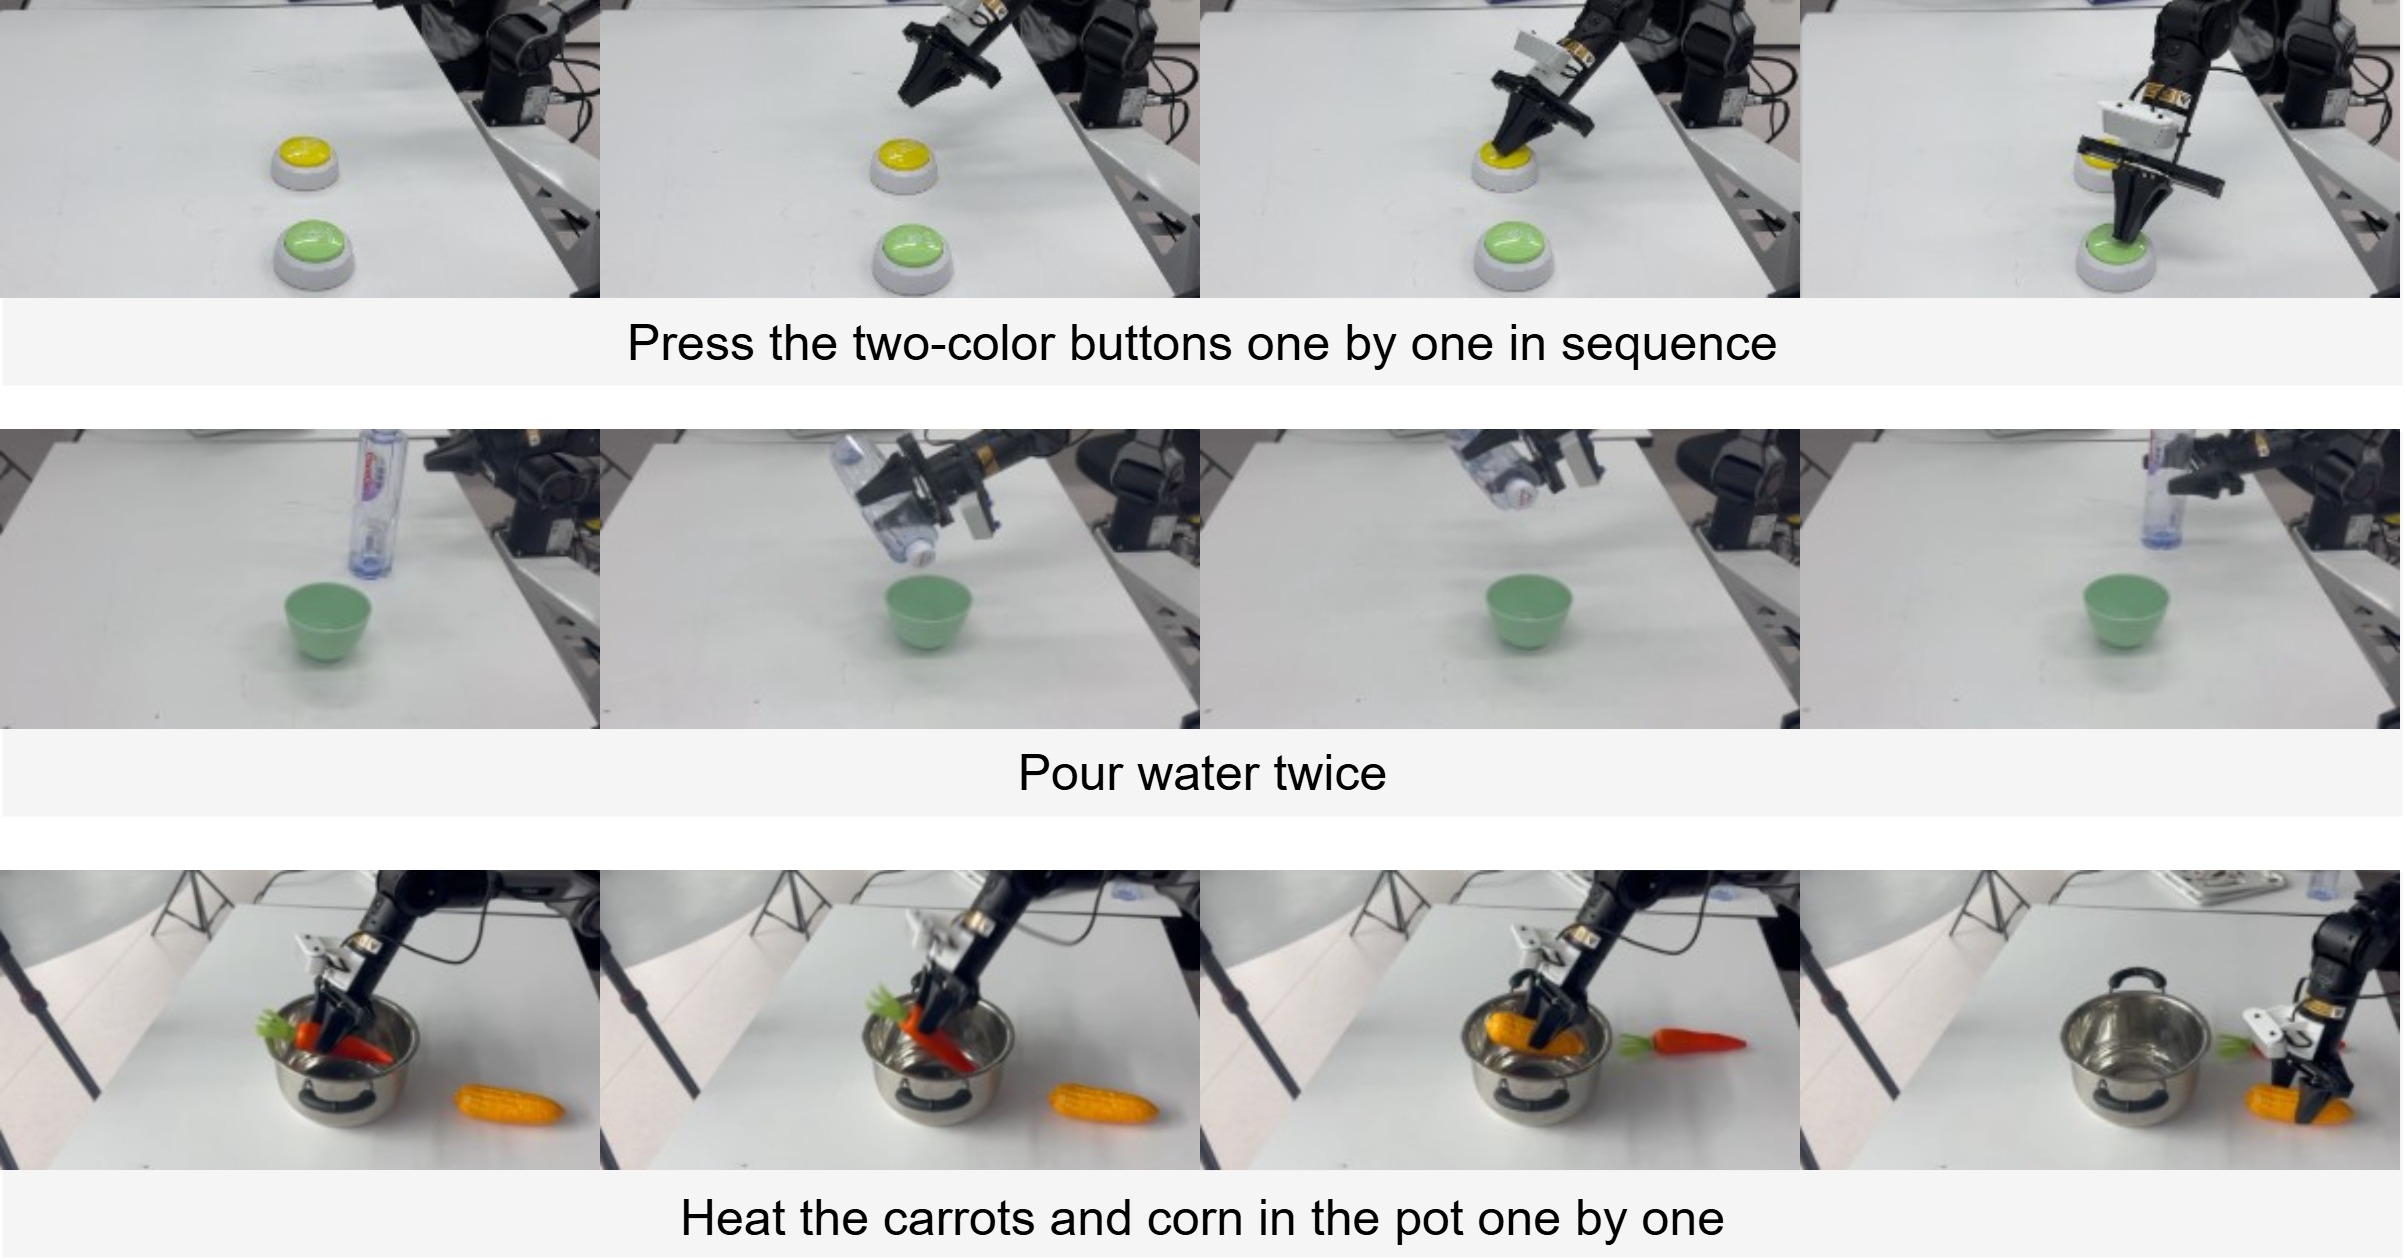
\includegraphics[width=\linewidth]{figs/real_demo_mem.jpg}
    \caption{Real-world tasks for multi-frame integration with the Cobot Magic robot: Press Buttons (top), Pour Twice (middle), and Heat Vegetables (bottom). Each task was evaluated over 20 trials.}
    \label{fig:dysta-real-mem}
\end{figure}

\begin{table}[t]
\centering
\caption{Real-world task accuracy (\%) on temporally dependent tasks for multi-frame integration. Each task is evaluated over 20 trials.}
\label{tab:real_mem}
\begin{tabular}{l|ccc|c}
\toprule
Method
& \makecell{Heat\\Vegetables}
& \makecell{Pour\\Twice}
& \makecell{Press\\Buttons}
& Average \\
\midrule
MemoryVLA
& $10.0$
& $25.0$
& $45.0$
& $26.7$ \\
ContextVLA
& $25.0$
& $40.0$
& $40.0$
& $35.0$ \\
\dysta{} (Ours)
& $\mathbf{35.0}$
& $\mathbf{75.0}$
& $\mathbf{65.0}$
& $\mathbf{58.3}$ \\
\bottomrule
\end{tabular}
\end{table}


\noindent\textbf{Implementation details} We use one static level. The ratio of static tokens is set to $0.9$, corresponding to $230$ static tokens and $26$ dynamic tokens. The number of observations is set to $20$, with a sampling interval of $20$ frames (1 frame per second), resulting in $750$ context tokens.


\noindent\textbf{Results} 
As shown in Table~\ref{tab:stove_res}, our method significantly and consistently outperforms all baselines on all objectives, with an average improvement of $24.5\%$.
Single-image methods such as TraceVLA almost always fail, since the task cannot be solved from the current observation alone, and visual traces provide only marginal additional benefit. 
ContextVLA underperforms due to non-learnable pooling observations, which may discard critical temporal and spatial details.
MemoryVLA presents the LLM backbone with only a single frame at each timestep, leaving multi-frame reasoning to a lightweight decoder; as a result, the LLM itself does not reason over multiple frames, which limits the model's capacity.
While these baselines have their own ways to reduce context length, they do so at the cost of information or model capacity. In contrast, our approach preserves all relevant visual information by reusing temporally persistent static tokens, enabling effective multi-frame integration within a limited context window.

\noindent\textbf{Real-world results}
As shown in Table~\ref{tab:real_mem}, \dysta{} achieved an average success rate of $58.3\%$ across the three real-world tasks, outperforming ContextVLA, the strongest baseline on average ($35.0\%$), by $23.3$ percentage points.

\subsection{Ablation Studies}

To validate the effectiveness of the proposed components, we conduct ablation studies on each of them, with results summarized in Table~\ref{tab:dysta-ablation}. From the second row, removing the contrastive learning objective leads to a noticeable performance degradation, as there is no longer an explicit mechanism to enforce temporal consistency in the static tokens. Performance also declines when the L2 static cache is removed and only a single-level static cache is used, as shown in the third row, highlighting the importance of the proposed multi-level caching design. Finally, replacing the learnable recache gate results in a further drop in performance, demonstrating the necessity of adaptive cache refreshing.

\begin{table}[t]
    \centering
        \caption{Ablation studies. \emph{w/o Contrast} removes the contrastive learning objective during training. \emph{w/o L2 cache} ablates the multi-level design by retaining only a single static cache level. \emph{Fixed step} replaces the learnable recache gate by forcing the refresh of the cache at fixed intervals. The refresh interval is set to match the average recaching interval of \dysta{} (first row).}
    \label{tab:dysta-ablation}
    \resizebox{\linewidth}{!}{
    \begin{tabular}{cccccc}
    \toprule
         & \multicolumn{2}{c}{visual matching} && \multicolumn{2}{c}{variant aggregation}  \\
         \cmidrule{2-3}
         \cmidrule{5-6}
         & PickCan & MoveNear & & PickCan & MoveNear \\
         \midrule
        \dysta{} & $\mathbf{92.7}$ & $\mathbf{88.8}$ & &$\mathbf{92.4}$ & ${81.0}$ \\ 
        w/o Contrast & $91.3$ & $84.6$ & &$91.6$ & $\mathbf{82.7}$ \\
        w/o L2 cache & $92.0$ & $85.0$ & & $91.5$ & $81.5$ \\
        fixed step & $87.7$ & $81.7$ & & $85.3$ & $74.8$ \\
    \bottomrule
    \end{tabular}
    }
\end{table}

\subsection{Visualizations}
We visualize the attention between the image and static/dynamic tokens across timesteps in Figure~\ref{fig:attention}.

\begin{figure}[t]
    \centering
    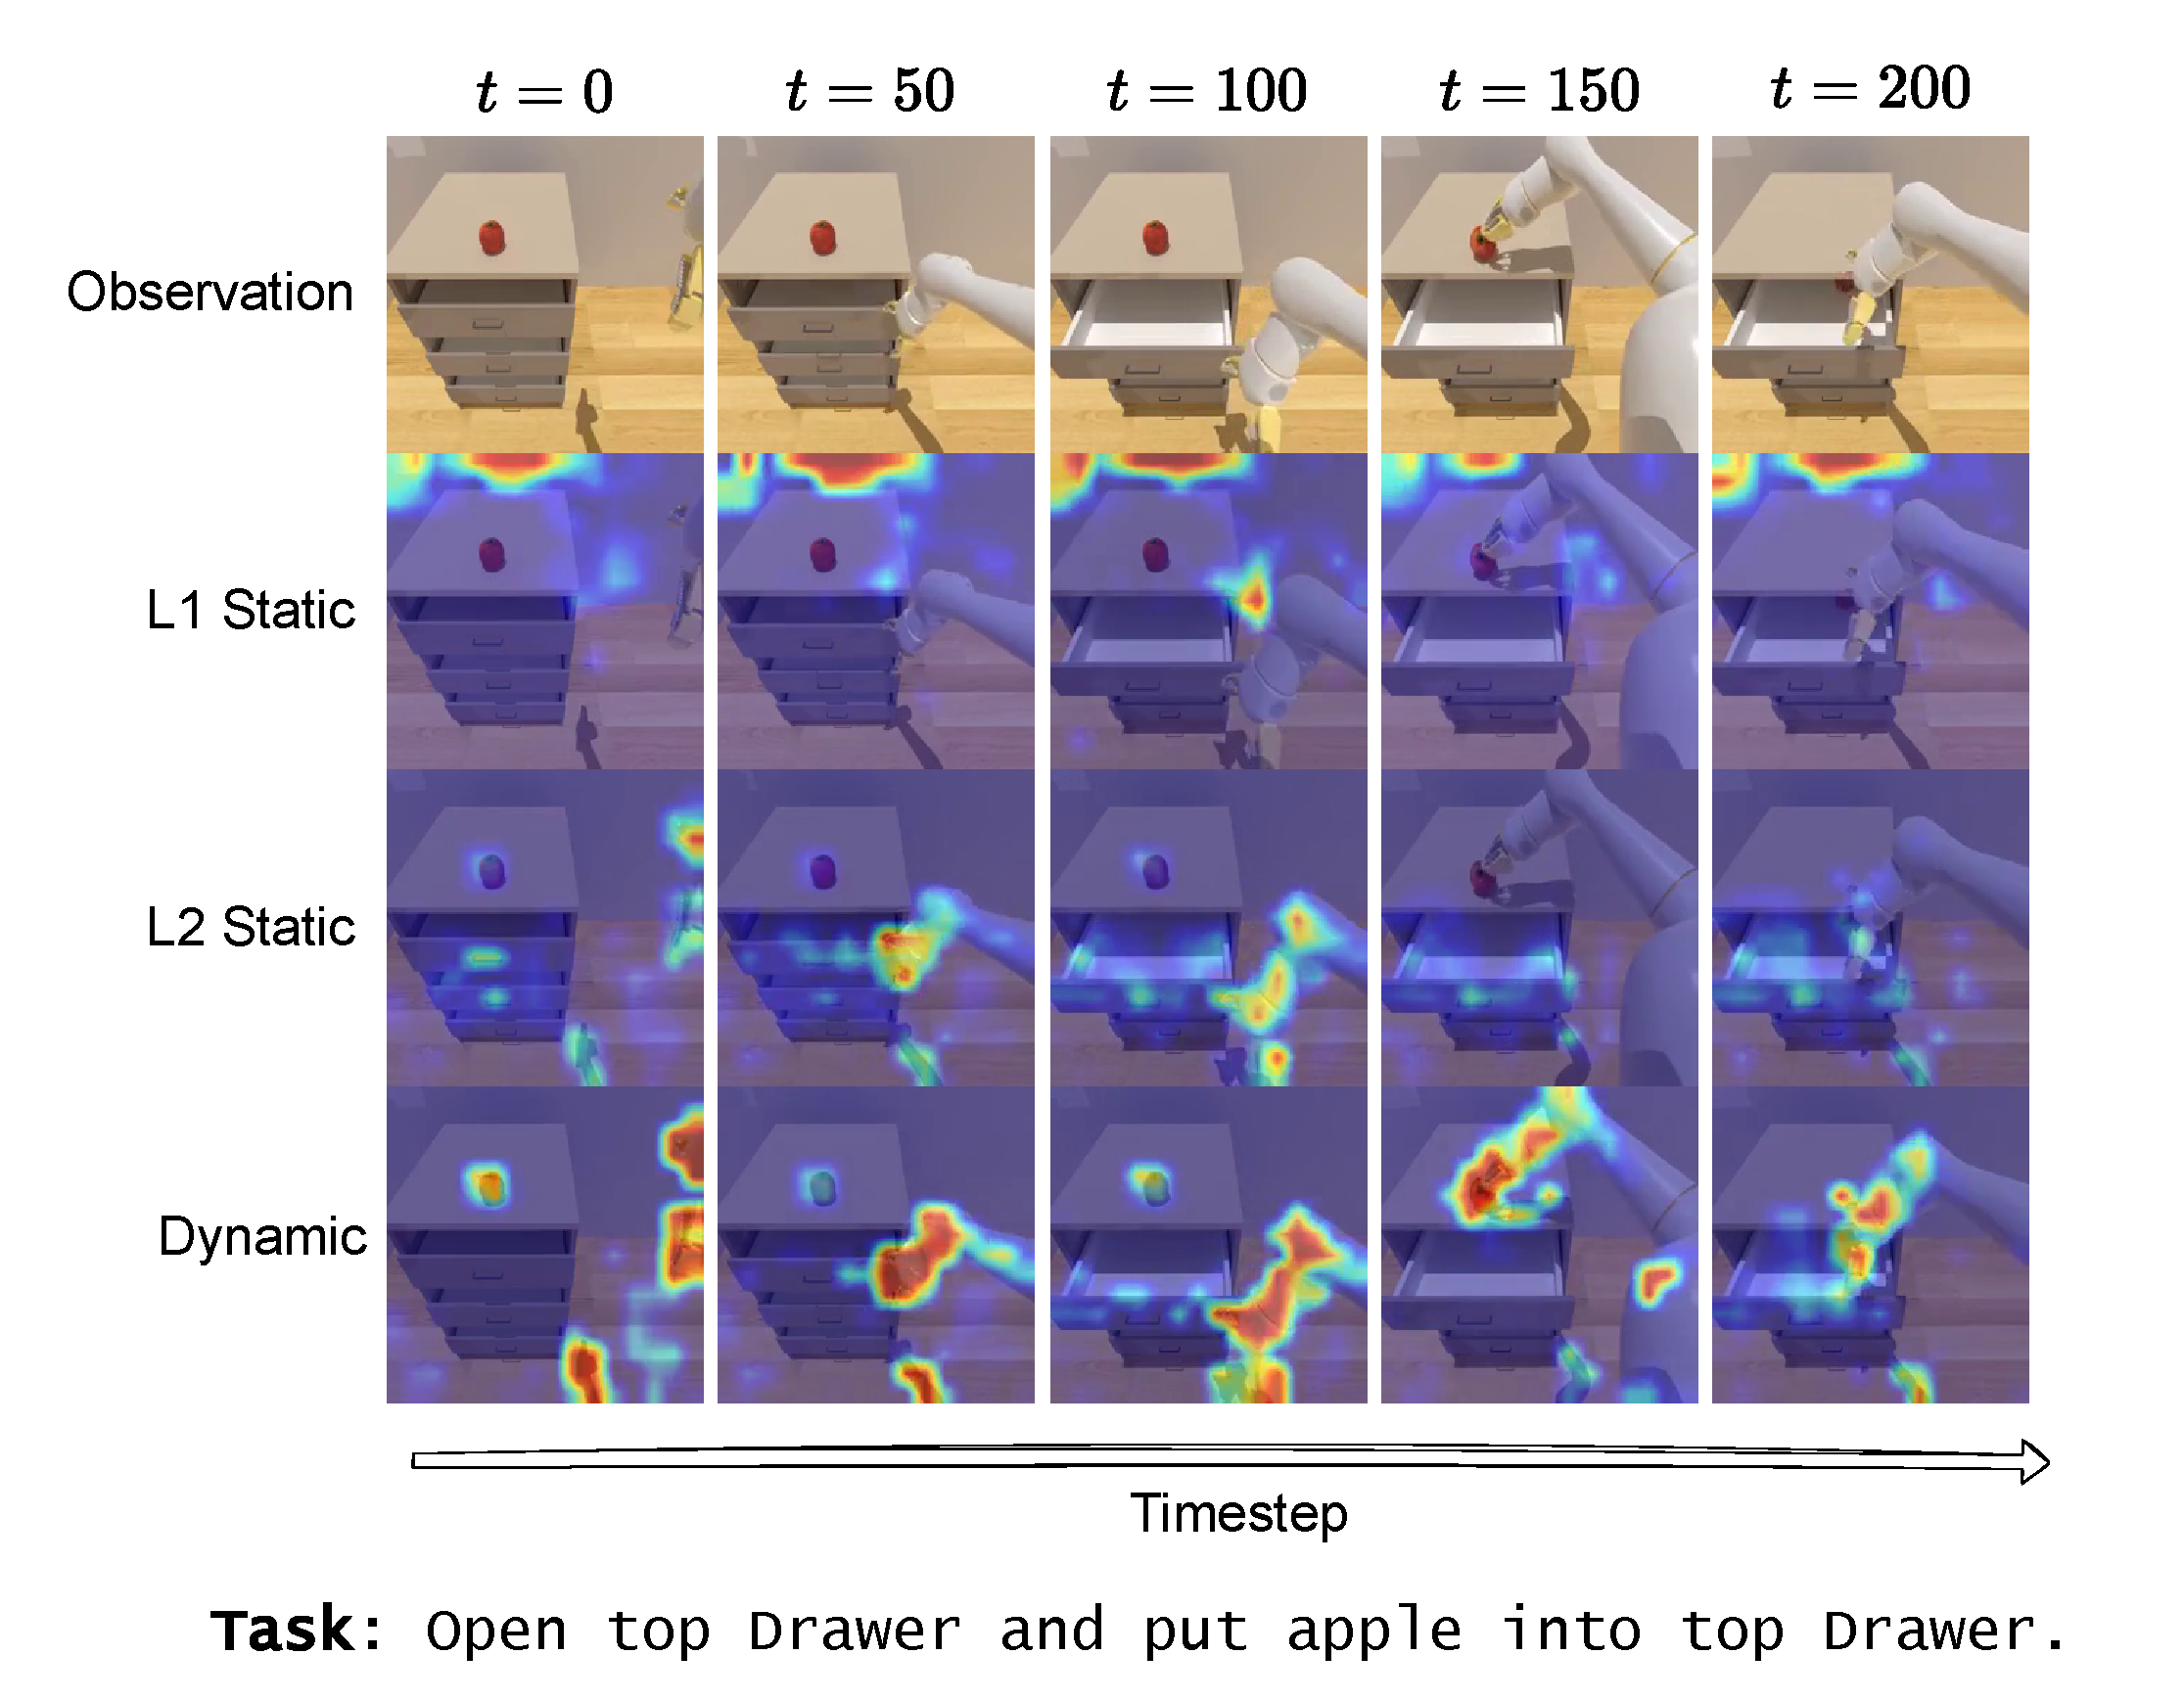
\includegraphics[width=0.9\linewidth]{figs/vis.pdf}
% \vspace{-15pt}
    \caption{Attention map visualization across time. For each token, we compute its last-layer attention to image patches and upsample the result to the full image resolution to produce a heatmap. Heatmaps are averaged over tokens of the same type and displayed by row (e.g., the Dynamic row shows the average attention heatmap of all dynamic tokens).}
    \label{fig:attention}
\end{figure}
Dynamic tokens consistently attend to movable objects, most notably the gripper (including its shadow) and the apple on the tabletop. This behavior aligns with their intended role of capturing temporally varying, action-relevant elements in the scene.

L1 static tokens, which are designed to represent the most persistent visual information, primarily focus on background and ambient regions. Their attention heatmaps are often strongest in areas without salient foreground objects. We interpret this behavior as L1 static tokens of shallow layers functioning as sink tokens, capturing coarse, global scene context rather than object-specific details. Importantly, their attention patterns remain highly consistent across timesteps, reflecting strong temporal invariance.

L2 static tokens exhibit intermediate behavior between L1 static and dynamic tokens. They attend more strongly to semi-static objects, such as the drawer, which typically remains stationary most of the time. At $t=0$ both drawer handles are highlighted, as either could potentially be moved. After the drawer is opened ($t>100$), the attention maps stabilize and remain focused on the drawer structure, indicating that these tokens capture object-level static information with moderate temporal persistence. The robotic arm is also highlighted at certain frames, which we attribute to its importance in the task and the need to preserve its appearance across timesteps.

